In this section, we will describe the machine learning techniques utilized as well as relevant background information regarding the
provided datasets and meterological use thereof.
\smallskip

\subsection{Convolutional Neural Networks}

Convolutional neural networks (CNNs) were initially introduced by Yann LeCun et al. in 1998 \cite{lecun-1998} and applied to the challenge of handwritten digit classification. However, the breakthrough for CNNs came later with the success achieved by Krizhevsky et al \cite{krizhevsky-2017}. in the ImageNet paper of 2012.
This work significantly advanced the state of the art of image classification.
\smallskip

CNNs are a class of deep learning models strongly capable of solving computer vision tasks. Unlike fully connected neural networks, which treat input data as a one dimensional vector, CNNs are designed to process higher dimensional data such as images.
This distinction enables CNNs to exploit more spatial relationships and patterns in visual data as opposed to a flattened vector where these patters are not recoverable.
\smallskip

Additionally Convolutional neural networks reduce the amount of parameters that are needed for each layer. This reduction is caused by parameter sharing.
In a traditional multi-layer perceptron weights exist for each connection while in CNNs a set of kernels are applied to the input. The kernels used in CNNs are small and are repeatedly applied across the input.
This reduces the amount of parameters the network has. 

\begin{figure}
  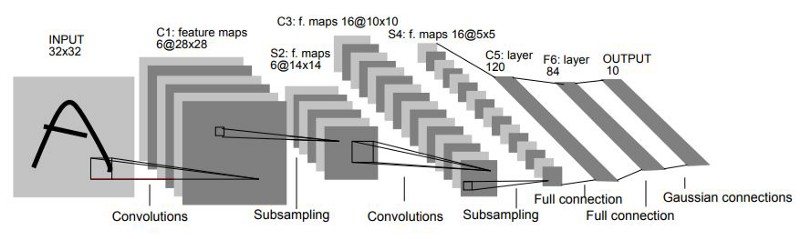
\includegraphics[width=8cm]{../images/cun.jpeg}
  \caption[short]{Architecture of LeNet-5: used for digit recognition and introduced by Yan LeCun \cite{lecun-1998}}
\end{figure}

\subsection{U-Net}
Semantic segmentation, the task of assigning a class label to each pixel in an image, is key to understand an image from a computer vision perspective.
This is the starting point for U-Net which was developed by Ronneberger et al. \cite{ronneberger-2015} to segment images from microscopes in biomedical applications.
U-Net is a fully convolutional architecture that provides accurate and detailed pixel-level predictions.
U-Net is specifically designed to capture both local and global context information.
The U-Net architecture gets its name from its U-shaped design (Figure \ref{fig:unet}), which consists of an encoder path and a decoder path.
The encoder path resembles a traditional CNN and serves the purpose of capturing spatial information
It is made out of multiple convolutional and pooling layers, where each convolutional layer extracts increasingly abstract features by convolving with learnable filters and applying the Rectified Linear Unit (ReLU) function \cite{relu}.
The decoder path, on the other hand, aims to recover the spatial information lost during the pooling and convolutional operations of the encoder.
It employs a series of transposed convolutional layers to gradually increase the spatial resolution.
The skip connections between the corresponding encoder and decoder layers help preserve fine-grained details that would be otherwise be lost during the encoding process.
U-Net is able to segment 2 dimensional images, however in some biomedical contexts 3D scans are used. To segment these kinds of inputs 3D U-Net was introduced by Çiçek et al. \cite{cicek-2016}.
3D U-Net is similar to 2D U-Net except instead of using 2D pooling and 2D convolution layers it uses it's 3 dimensional counterparts. Authors such as Brodehl. \cite{predictionLightning} have shown that
the depth dimension in a 3D U-Net can be replaced by the time dimension which leads to capturing time based context information.

\begin{figure}
  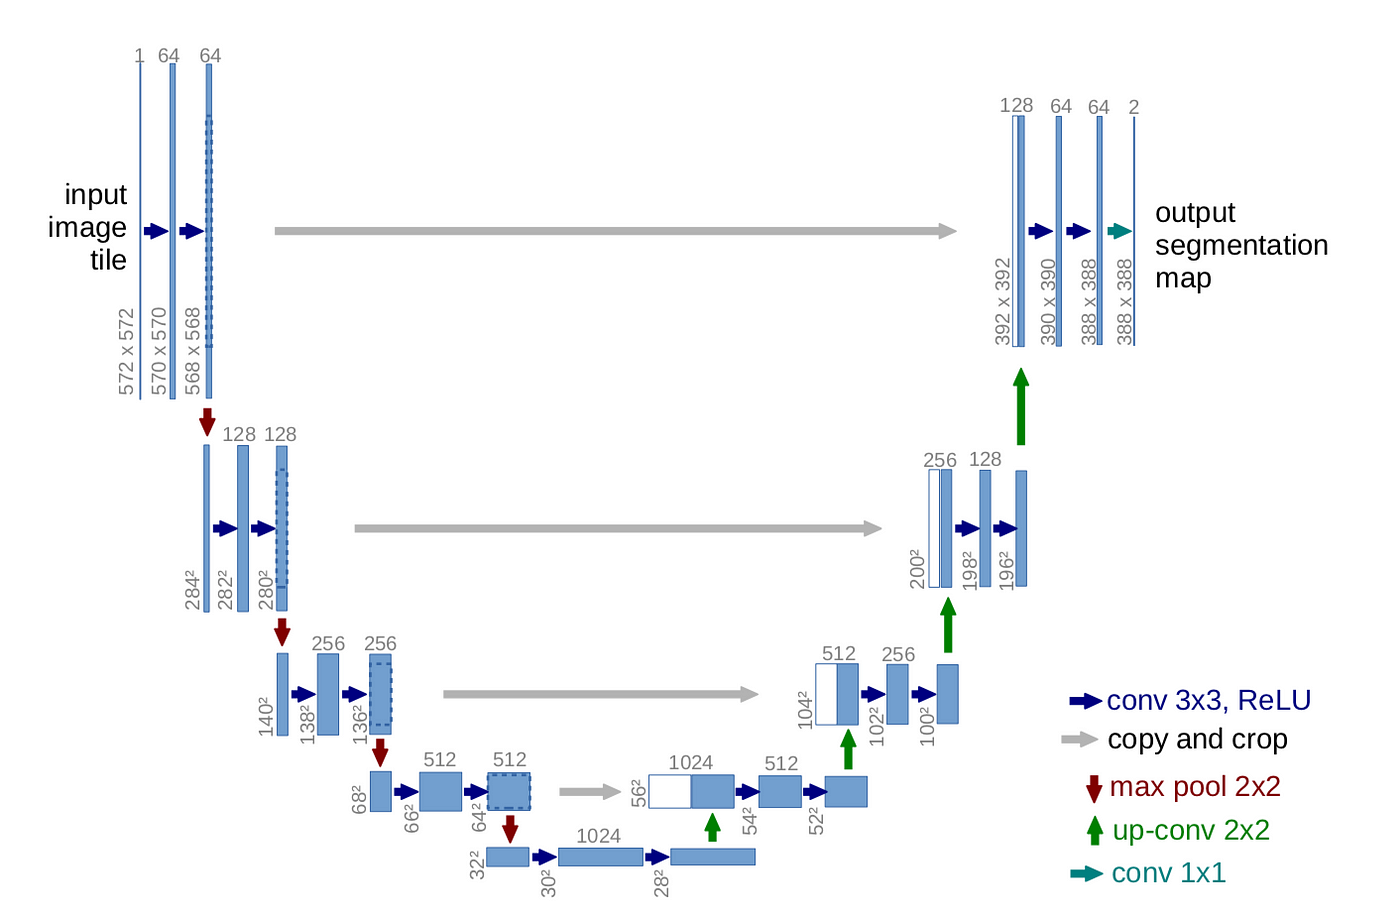
\includegraphics[width=8cm]{../images/unet.png}
  \caption[short]{U-Net architecture, encoder and decoder sections of the model form the U structure. Encoder Passes context information to the decoder through \textit{skip connections}. \cite{ronneberger-2015}}
  \label{fig:unet}
\end{figure}

\subsection{Convolutional LSTM}
%As mentioned in the related works, the LSTM model, introduced by Hochreiter et al. \cite{lstm}.
%The improvement of this recurrent neural network design over prior designs is that a long term memory path was introduced.
%The long term memory path can be operated on by the input sequences, the operations that are performed on the long term memory
%depend on \textit{gates}.
%There are two gates that affect the long term memory: the input gate which decides which new information will be added and the forget gate, which decides how much will be forgotten.
A traditional LSTM operates with vectors \cite{lstm}, this would mean that to process images in a LSTM these would need to be flattened to a vector, most spatial information would be lost. This is why Shi et al. introduced ConvLSTM \cite{convlstm}.
Which replaces the learnable vectors in the LSTM with kernels, and the operations become convolutions.
The equations of the ConvLSTM cell are below (equation 1-4). Each ConvLSTM cell produces a short term memory $ \mathcal{H}_{t}$ and a long term memory $\mathcal{C}_{t}$,
the output after passing all of our sequence to the model is the short term memory $\mathcal{H}_{t}$. 
The formulas can be explained relying with the use of activation functions $\sigma$ and $tanh$, sigmoid and hyperbolic tangent.
The sigmoid function maps any $x$ between 0 and 1, values between 0 and 1 are used here as the \textit{fraction of information that is added or removed}.
On the other hand the hyperbolic tangent function maps an input $x$ between $-1$ and 1. Therefore when the sigmoid activation represents the fraction or percentage of information being added or removed from for example the
long term memory while the $tanh$ function is being used to normalize the information itself between 0 and 1.
Take for example the equation for the forget gate (equation 2), noting that $*$ notates a convolution operation.
The result of this equation is a matrix with values between 0 and 1 due to the sigmoid function.
The $f_t$ is used in equation 3, it is used to calculate the element wise multiplication notated $\odot$
with the previous long term memory. This allows only a fraction of the long term memory, to continue into the output of the
current cell and further cells in the unrolled Convolutional LSTM. This is why it is called the forget gate. 

\begin{equation}
  i_{t} = \sigma\left(W_{xi} * X_{t} + W_{hi} * H_{t-1} + W_{ci} \odot \mathcal{C}_{t-1} + b_{i}\right)\\
\end{equation}

\begin{equation}
  f_{t} = \sigma\left(W_{xf} * X_{t} + W_{hf} * H_{t-1} + W_{cf} \odot \mathcal{C}_{-1} + b_{f}\right)
\end{equation}

\begin{equation}
  \mathcal{C}_{t} = f_{t} \odot \mathcal{C}_{t-1} + i_{t} \odot \text{tanh}\left(W_{xc} * X_{t} + W_{hc} * \mathcal{H}_{t-1} + b_{c}\right)
\end{equation}

\begin{equation}
  o_{t} = \sigma\left(W_{xo} * X_{t} + W_{ho} * \mathcal{H}_{t-1} + W_{co} \odot \mathcal{C}_{t} + b_{o}\right)\\
\end{equation}

\begin{equation}
  \mathcal{H}_{t} = o_{t} \odot \text{tanh}\left(C_{t}\right)\\
\end{equation}

\subsection{Attention}
The concept of the attention mechanism in machine learning comes from Bahadanau et al. \cite{bahdanau-2015}. The authors were investigating how to assign different levels of importance to each input in a sequence to sequence model.
Usually attention is computed through a shallow multi-layer perceptron (MLP) since it is expensive to add attention to a model.
However this shallowness is not enough when it comes to computer vision models. Because we are dealing with inputs that are images the amount of connection becomes $(h\times w)^2$
due to the fact that every neuron in the input layer must be connected to the neuron in the output layer.
To address this issue, Axial Attention was introduced by Ho et al. \cite{DBLP:journals/corr/abs-1912-12180} as a means of alleviating this problem.
Axial attention simplifies the computation of attention by exclusively considering the adjacent row and column, thus mitigating the exponential growth of parameters.

\subsection{Radar Data}
Radar instruments are employed to measure precipitation levels within a given area.
These devices operate from ground level and emit microwave pulses while rotating.
As these pulses encounter atmospheric particles, they disperse in various directions.
A portion of the energy emitted by the radar is reflected back and recorded.
By employing the relationship between speed, time, and distance, the radar can determine the particle's proximity to itself.
The quantity of energy that returns to the radar following interaction with precipitation is termed \textit{reflectivity} denoted by $Z$.
To assess the rainfall rate in millimeters per hour, the Marshall Palmer Relationship, \cite{marshall-1948} is utilized to convert reflectivity factor.
Meteorologists often prefer to use decibels relative to $Z$ as a more convenient unit.
This unit expresses reflectivity relative to a 1 millimeter drop within a cubic meter of volume ($Z_0$) \cite{rogers-1976}.

\begin{equation}
  dBZ = 10 \times log_{10}(\frac{Z}{Z_0})
\end{equation}

See table \ref{tab:data} for a table with dBZ values and their corresponding meterological interpretation.
The range of a radar extends to a couple hundred kilometers from their origin which means that to observe a larger area a group of radars
can be combined to form a composite radar image (see figure \ref{fig:radsource}). 


\subsection{Satellite Data}
Satellites play a crucial role in meteorology as they provide valuable observations of the Earth from above.
Geostationary satellites orbit the earth at the same speed as the planet's rotation on it's own axis, which allow them to be fixed relative to a given longitude.
This class of satellites orbit the earth at an altitude of $\approx 35786 km$.
Worldwide coverage can be achieved by deploying multiple satellites, for example EUMETSAT operates MSG satellites for Europe, NOAA operates GOES satellites for the Americas and the Himawari satellite is operated by the Japan Meteorological Agency, which covers the Asia-Pacific region.
Focusing on Meteosat-10 satellite from which we obtain our data, this satellite produces a scan every 15 minutes.
We obtain 11 satellite images corresponding to different spectral channels (see figure \ref{fig:satchannels}). Three main types of channels are available: visible, infrared and water vapour channels (See table \ref{tab:channels}). 
Visible channels are measured by the satellite when radiation from the sun reflects on the earth's surface, infrared channels on the other hand receive radiation emitted by the earth and clouds allowing for imagery even at nighttime. The wave vapour channels on the other hand, capture radiation emitted
by water vapour in the upper troposphere.
